% !TeX root = ../main.tex
% Add the above to each chapter to make compiling the PDF easier in some editors.

\chapter{Discussion}\label{chapter:discussion}

The last chapter focused on results derived from the BERTopic topic model and analyzed them in 
detail. This chapter focuses on interpreting these results in a broader context and discusses this
thesis's limitations and future work. 

\section{Interpreting the results in a broader context}

Having the results analyzed in detail, this section focuses on interpreting these results in a more 
expansive concept. It aims to answer the remaining research questions about parties and their election 
agendas and compare the topic model results with related research. This section aims to answer the third 
research question.

Analyzing the 1000 topics individually, one can realize that these topics cover lots of topics, 
which also mirror the parties' agendas and public statements on both ruling and opposition ranks. 
These resulting topics cover a wide range of strategies utilized in the months leading up to the 
election, including those used by the opposing and ruling blocks to strengthen their position against each 
other. Specifically, the topics span various issues such as the rule of law, the constitution, the 
economy in general, both foreign and domestic policy, mottos of election campaigns, and many more.

The focus starts with the opposition rank. The Nation Alliance of six parties was formed in 
2022 mainly because it focused on restoring the rule of law. They introduced the so-called 
´Strengthened parliamentary system', a form of government that aims to return to the parliamentary system 
from the presidential system that has been in effect since the 2017 referendum. Without going into detail, 
the Nation Alliance seeks to limit the executive branch's powers by empowering the legislature, the 
Turkish parliament, to prevent the slide to autocracy in the future \parencite{edgar_sar_opposition_election_agenda_2023}.

One can realize the importance of political figures in Turkish politics by looking at the top topic 
model results. That is why the opposition's candidacy has also been a hot topic for months, with the 
view that only a strong candidate could prevail against Erdoğan. The topic of opposition candidacy, 
being one of the top topics, supports that idea. There are almost more than 12 topics regarding political 
figures in the top 100 topics, which make up more than 10\% of all tweets analyzed. These 12 topics refer 
to Kılıçdaroğlu, Erdoğan, Meral Aksener, mayors like Ekrem İmamoğlu and Mansur Yavaş, 
ministers like Mustafa Varank.

Introducing a ´Strengthened parliamentary system' by the Nation Alliance focuses on ensuring an independent 
and impartial judiciary, reforming public institutions, and systematically preventing human rights 
violations \parencite{edgar_sar_opposition_election_agenda_2023}. One of the mottos of the opposition 
party CHP highlighting this issue was \textit{'hak, hukuk, adalet'}, which translates to rights, law, and 
justice. There are more than four different topics in the topic model results, and they focus on the 
constitution, the regulations and trials, and the imprisonment sentence for İmamoğlu, the mayor of Istanbul. 
Most of the topics in this section refer to human rights violations and dependent and biased judiciary. 

Around four topics in the topic model results relate to the imprisonment sentence for the mayor of 
Istanbul, İmamoğlu, and contain more than 550 thousand tweets in the dataset. The imprisonment sentence 
just before the elections and the justification of it are solid examples of a biased judiciary. For context, 
the first local election in Istanbul was canceled, and it happened again. İmamoğlu won both of the 
elections, with a significant difference in the second one, gaining support. In France in 2019, 
İmamoğlu stated in a conference that the government canceled the elections to try to win in the second 
round, where they used extensive state resources and polarized the people. Süleyman Soylu, who was the 
minister of the Interior, called Imamoğlu a fool for complaining about Turkey to the EU. 
On the same day, İmamoğlu called the one(s) who canceled the elections fools and said Soylu should focus 
on them instead \parencite{bbc_imamoglu_dava_2022}. The court sentenced İmamoğlu to over two years 
imprisonment for calling Supreme Elec­toral Board members fools \parencite{aktürk_imamoglu_dava_2022}. 
Because the sentence had not yet been upheld, it was feared that if İmamoğlu were selected as the 
opposition candidate, the government would use his sentence to drop his candidacy, which would weaken 
the opposition ranks.

Another hot topic that the opposition criticized in the ruling bloc is the economic condition of the country 
and the ongoing hyperinflation in the months up to the elections. The unexpected earthquake made the top 
of the cake with massive economic repercussions \parencite{cevik_aksoy_turkey_earthquake_2023}. Just 
before the elections, the official infla­tion rate reached a 24-year high of more than 85\%, 
and other unofficial sources show even more than 100\% \parencite{edgar_sar_opposition_election_agenda_2023}. 

The topic model results cover topics regarding the economy, exchange rates of the dollar and Euro to the 
Turkish Lira, the inflation rates, and the accused missing 418 billion dollars from the state treasury. 
Although these topics do not comprise the trending topics, at least five related topics can be found in the 
topic model results.

The exchange rate from the dollar to the Turkish Lira was 2 in 2013, 4,5 before the 2018 elections, 
increased to 8,5 till September 2021, and 20 before the May 2023 elections. The government has been accused 
of selling reserves from the treasury to keep the exchange rate low and depending on foreign money from the 
Gulf states and Russia \parencite{edgar_sar_opposition_election_agenda_2023}. As of 2024, the exchange 
rate is 30, marking an increase of more than 500\% in just five years.
The government also kept the central banks' interest rates low. With the hyperinflation and depleted 
central bank reserves, the Turkish Lira devaluation was inevitable.

The main motto of the opposition party CHP and its candidate Kılıçdaroğlu during the election campaign 
was \textit{'Sana Söz yine baharlar gelecek\ldots'}, which translates to 
\textit{'Promise, the spring will come again\ldots'}. 
The motto itself was also used in various campaign videos, and it originates from a song and symbolizes 
hope. The topic around that motto can also be found in the topic model results.

In the election month, disinformation on social media was on the rise. The campaign video of Kılıçdaroğlu 
based on the motto was a target of this disinformation, which was modified. An old clip of terrorists 
applauding and keeping rhythm was cut and added at the end of the campaign video and released on social 
media. In order to mobilize nationalists, the government bloc was already accusing the opposition parties 
of having a relationship with terrorists, and with this video becoming a trend, that thought of view 
skyrocketed. Even President Erdoğan showed the video during one of his rallies, which helped spread the 
disinformation \parencite{ogras_disinformation_chp_pkk_2024}.

Another topic that is deeply analyzed and discussed in this thesis is the migration policy. Since Turkey has 
a vast incoming migration, making Turkey the top host country for refugees in the world, the topic was also 
one of the trending topics of the May 2023 elections on social media. While the ruling bloc is taking a 
sympathetic approach to refugees, portraying them as religious brothers, the opposition bloc opposes the 
long-term settlement of refugees, mainly Syrians, and it promises to send the (illegal) refugees back to 
their countries \parencite{berk_esen_turkish_politics_2023}. The topic model results cover these points 
by at least four separate topics. The top topic focuses specifically on Syrians, but they do not make 
the top 50 topics.

The importance of the earthquake and how it affected the elections is discussed in detail in this 
thesis. Since the earthquake was a national disaster, it played an essential role in unifying the 
people in a highly polarized society. The role of unification in times of crises has also been the 
approach of the second biggest opposition party \ac{IyiP} and its leader, Meral Akşener. She supported 
the idea that the earthquake was not open for a political debate and stayed silent in the first days. 
However, the to-be opposition candidate at that time, Kılıçdaroğlu, was present from day one in the 
catastrophe zone, leading a political campaign that criticized Erdoğan and his officials
\parencite{cevik_aksoy_turkey_earthquake_2023}. These two different approaches revealed profound 
divi­sions in the Nation Alliance, which continued after the selection of Kılıçdaroğlu as the joint 
candidate. These divisions are also some of the main reasons that push the topic of the earthquake 
and the opposition's candidacy, making them trending topics. 

Foreign policy is another aspect to analyze. \textcite{edgar_sar_opposition_election_agenda_2023} remarks 
that foreign policy has often been seen as a part where the opposition has mainly struggled to 
establish a unified approach. Şar presents two reasons for that. The first one is that the parties in the 
Nation Alliance have different perspectives on how foreign policy should be changed or directed. 
Secondly, Şar states that foreign policy is typically perceived as having minimal to no impact on the 
voting patterns of the Turkish electorate, which gives the opposition block the motivation to focus on 
considerably more critical areas.

However, there is another argument that the success of the ruling bloc on foreign policy might have 
boosted the approval rates of Erdoğan and the People Alliance in the months up to the elections. 
Erdoğan achieved this by portraying himself as an influential statesman, a mediator in international 
conflicts, for instance between Ukraine and Russia, and a reliable defender of national 
interests \parencite{cevik_aksoy_aydin_turkey_after_elections_2023}. Approval rates of approaches like 
this make it more complicated for the opposition block to suggest a different approach and leave them 
with only the choice of supporting the current foreign policy.

There are more than five different topics in the model results that cover foreign policies, the 
first being in the top 50 topics and about Russia and Ukraine. Other topics cover Germany and the 
European Union, the visa problems, NATO and the USA, and the conflict between Azerbaijan and Armenia.

\textcite{edgar_sar_opposition_election_agenda_2023} stated in February that for the Nation Alliance to 
secure a governing position, it must have first rallied an electoral majority through persuasive efforts 
with voters. Despite being fully aware that achieving this requires a successful electoral strategy, the 
alliance had, until February, focused more on developing its vision for the post-election period, rather 
than discussing and agreeing on a joint candidate, for instance. This highlights the main reason for the 
failure of the opposition bloc.

% Ruling ranks:
The focus of the analysis continues with the ruling ranks. It is essential to mention again that 
foreign policy has been one of the most influential topics that the ruling block sees as a success 
element, specifically after 2022, being a mediator in international conflicts, for instance, between 
Ukraine and Russia. The government also portrayed itself as defending national interests, increasing 
decisive military power in foreign countries. Mili­tary operations in Libya, Syria, Iraq, and the 
South Caucasus, military bases in Somalia and Qatar, and a growing domestic arms industry are solid 
examples \parencite{cevik_aksoy_turkey_earthquake_2023}. Another example was the Turkish government 
vetoing Sweden's accession to NATO. 

However, in January 2024, after US President Joe Biden sent a letter to Congress expressing the 
selling of F-18 fighter jets, the Turkish government approved Sweden's accession to 
NATO \parencite{euronews_sweden_f18_2024}. One can notice various topic model results covering 
these issues, going deep as addressing specific military operations, for instance, one done in Syria.

The relationship between Turkey and other countries in Gulf states and Russia has also been improving 
under this government, where Erdo­ğan uses foreign connections to gain financial and economic deals, 
keeping the 22-year AKP machine running \parencite{cevik_aksoy_aydin_turkey_after_elections_2023}.

While projecting power internationally, the government successfully creates ´foreign enemies', 
presenting itself as safeguarding national interests. With the help of the control of the mainstream 
media, Erdoğan's command of the Turkish right and his ability to mobilize religious nationalist 
voters can not be denied. Looking at the top 100 topics of the topic model results, one can find more 
than nine topic representations covering the previously mentioned issues. 

Three of these clusters cover topics around terrorism and the accusation of a relationship of parties 
with terrorist organizations. These are solid examples of why the opposition block had to convince 
people they were not affiliated with any international or terrorist organizations. 

At least three clusters in the top 100 topic model results present topics related directly to 
President Erdo­ğan. While two of them show support for Erdo­ğan, the other prays for Erdo­ğan. A 
representative tweet for the latter topic would be \textit{'May God keep Erdo­ğan in power.'}. No 
less than two clusters in the top 100 topic model results cover nationalism, and at least one of them 
is directly related to the \ac{MHP} since its name includes nationalism. The representative tweets 
in this cluster demonstrate voting for Erdo­ğan and \ac{MHP} in the first round of the elections, 
mainly aiming to increase \ac{MHP}'s power in the parliament.

The cluster on the 40\. place of the topic model result is about trust in the state, which would 
mean supporting the governing block. An example representative tweet here is 
\textit{'We trust our state, our goal is to serve our state.'}. That is a solid example of how the 
ruling block successfully merged the state and the party. The merger of the state and the government, 
the unfair elections, and many other reasons sum up why the government can be called a competitive 
authoritarian regime, a concept in Comparative Politics defined by \textcite{levitsky_elections_2002}.

One of the main differences between the opposition and the ruling block is their emphasis on 
religion. The opposition block offers a secularist approach to religion. For instance, the opposition 
aims to cut some costs from the Ministry of Religious Affairs, which has a yearly budget of over 
2 billion dollars, exceeding many other ministries. The ruling block, on the other hand, emphasizes 
tradi­tional Islam and family values, and uses religion wherever it can 
\parencite{cevik_aksoy_aydin_turkey_after_elections_2023}. Kılıçdaroğlu's religious identity, 
Alevism, also does not contribute to convincing religious conservative voters, which diverges 
from the traditional Sunni Islam.

An essential argument for why some people vote for the governing block is the guarantee of continuity 
and stability. According to \textcite{cevik_aksoy_aydin_turkey_after_elections_2023}, the governing 
block was socio-politically and ideologically more coherent than the oppo­sition and succeeded 
in presenting itself like that. At least one cluster in the top 50 topic model results also 
supports the argument.

Finally, it is essential to mention the motto of the ruling block, which was 
\textit{'Türkiye Yüzyılı'}, which translates to \textit{'Turkey's Century'}. One of the clusters 
in the top 5 topic representations that include at least 2,7 million tweets also covers this topic. 
The ruling block used this motto, which highlights the 100\. year of the Turkish Republic, also 
presenting a website\footnote{\url{https://turkiyeyuzyili.com}}. The website includes many 
(mega) projects from more than 17 categories, some covering more than 65 projects. 
These projects cover what the ruling block has done till the elections and their aims for the 
following century.


% Beyond the Data: Global and Political Insights
% refer to polutus, sentiment analysis etc.
% - "How do the Twitter discussions about the ruling party and the opposition during the election 
% lead-up reflect and compare to their respective election agendas and public statements?"
% agendas
% TODO: already a little bit mentioned in the results part

\section{Comparing the results with relevant research}

This section aims to compare and analyze the results of this thesis with other relevant research and 
their results and answer the last research question. While the first focus lies on research relevant 
to Turkish elections, the second focus is on research in other countries.

The most important paper for this thesis would be from \textcite{secim2023}, with which the dataset 
of this thesis was published. The research discovered that the trending topics of the dataset from 
July 2022 to October 2022 reflect important events from sports, political debates, or TV, and 
suggests that almost half of the top five daily trends are generated by coordinated attacks. 

\begin{figure}[h!]
    \centering
    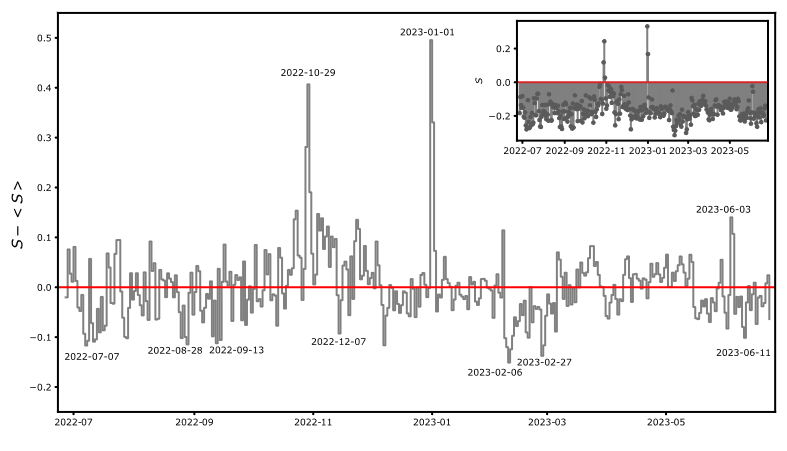
\includegraphics[width=\linewidth]{figures/sentiment_plot.png}
    \caption[Daily sentiment analysis]
    {Daily sentiment, and sentiment difference from the mean. S and <S> stand for sentiment and mean 
    sentiment of tweets. The figure is taken
    from \textcite{turkishbertweet_2023}}\label{fig:sentiment_analysis}
\end{figure}

The second research from the same chair is from \textcite{turkishbertweet_2023}, which developed its 
own language model called TurkishBERTweet, which has been trained on almost 900 million tweet data 
from 2009 to 2022. The chair applies the LLM on the \#Secim2023 dataset for sentiment analysis of 
336 million tweets. The \autoref{fig:sentiment_analysis} presents daily sentiment and the sentiment 
difference from the mean of the tweets from July 2022 to June 2023 in one graph. One can realize some 
intense sentiment values in the figure. For instance, 29 October and 1 January have extreme levels of 
positive sentiments. 29 October is the day of the proclamation of the Turkish Republic, and the latter 
is New Year's Eve.

On the other hand, 6 February and 27 February mark high levels of negative sentiments. Both of the 
dates are about the earthquake, the first one being the day of the earthquake and the latter about 
the day Erdo­ğan visited earthquake regions and asked for forgiveness. On the same day, a trend on 
Twitter started against Erdogan's ask for forgiveness. This thesis's topic model results also present 
the earthquake topic as one of the most spoken issues.

The following two research reports are based on an EU-supported 
project\footnote{\url{https://cordis.europa.eu/project/id/101082050}} implemented by Koc University 
in Istanbul.

The first report, by \textcite{politusanalytics_1_2023}, presents sentiment analysis, emotional analysis, 
and idealogy analysis of the social media data, which includes in sum 310 million tweets. 

The results propose that the primary emotion of the results was anger, highlighting the general 
correlation between tweeting and being angry. Naturally, after the 6 February earthquake, the 
dominant emotion was sadness, while happiness reduced sharply. Hope increased dramatically in the 
week of the candidacy announcement of Kılıçdaroğlu, the results show. Desperation was examined in 
the opposition ranks more significant than the ruling block ranks, losing its significance only 
after the candidacy announcement and continuing its trend until the elections. While confusion 
levels among the ruling ranks remain stable in 2023 until the elections, it is unstable among the
opposition ranks with ups and downs, underlining the uncertainties with candidacy and other joint 
approaches. 

The report also underlines the relationship of anger with topics like human rights, the economy, 
and justice. These mentioned points support the results of the thesis' topic model results. 
The emphasized emotions demonstrate why some of the discussed topics in this thesis were trending 
during the months up to the election.

The report also analyzes specific topics' trends between January and May. The results suggest 
similar results to the thesis' topic results, where the earthquake changed the trend of the 
discussed topics on social media in February, taking the top place. After March, the focus lies 
more on the upcoming election and other political discussions. Other topics cover the economy, 
the constitution and the regime, foreign policy, and the Kurdish community, once more akin.

The second report, by \textcite{politusanalytics_2_2023}, was published between the first and 
second rounds of the May 2023 elections and aimed to continue the first report. The analysis 
starts with the approval rates of Kılıçdaroğlu and Erdoğan between January and May 2023, according 
to Twitter, with the use of three different models. The result of the analysis suggests that the 
support rate of Erdoğan was, in general, higher than that of Kılıçdaroğlu, in which the gap between 
them peaked at the end of April.

The comparison with relevant research continues with different research papers that have used BERTopic 
or another topic model to analyze data from various domains, where the focus of this thesis remains 
as the political domain. 

To start with, the first research that leveraged the power of different BERTopic models suggests that 
BERTopic results seem more specific than other topic models 
\parencite{topic_model_comparison_bertopic_2022}. This thesis also underlines that if the default 
values of parameters are not manually changed heavily so that the minimum size of clusters gets 
enormous, the BERTopic results appear specific. More than 7000 in the first approach and more than 
1000 topic cluster results in the second approach are substantial examples. Furthermore, if one 
analyzes the topic clusters carefully, it is realizable that there are many similar topics. 
Nevertheless, these similar topics appear to differ at least in one part in many cases, for instance, 
one topic being about conservative nationalism and the other Kemalist nationalism. However, it is 
essential to highlight that analyzing the results usually takes more work when the number of topic 
clusters reaches more than several hundred.

The following research by \textcite{ilyas_brexit_topic_modeling_2020} used the LDA topic model to 
analyze the trend of topics related to Brexit on Twitter. The research had a similar research question 
to this thesis to determine if the discussed topic on Twitter was real-life events. The research 
analyzed a three-month period and found that their results highly represented the actual events. 
These topics cover speeches of Boris Johnson and the Queen, the deal with the EU, and events around 
the parliament. All of these events were trending topics during that period. 

Although the analyzed time period in this thesis is four times more than this research, this thesis 
also found a correlation between real-life events and the discussed topics on Twitter. Some of the 
topics that this thesis found are the earthquake, the prison sentence of Imamoğlu, and the election 
results or events that happened during the elections. This correlation suggests that politicians 
can use social media data and their analysis to better understand public opinions and determine 
their policies respectfully.

The following two research focus on German elections and the topics around them on social media. 
The first one by \textcite{stier_germany_election_2018} focuses on the German federal election 
campaign in 2013 and trains a Bayesian language model to identify topics from politicians' posts 
and their comments. The research suggests that the messages from politicians and their audiences 
prioritize different topics. As future work, this thesis could also separate tweets from the 
politicians and voters and analyze the corresponding results accordingly to find the difference 
between them in Turkish politics. \textcite{stier_germany_election_2018} discovers that the top six 
topics covered on Twitter were political debates, polity, law and order, coalition formation, 
campaigning, and the labor market. All of the mentioned topics in the 2013 German elections were 
similar to these thesis findings of the 2023 Turkish elections. However, unlike the 2023 Turkish 
Twitter political discourse, in German political discourse, the following topics are very short in 
volume: economy, currency and Euro, migration and integration, and foreign policy. 

The following research by \textcite{bertopic_twitter_german_politics_2022} is based on a thesis where 
BERTopic and other topic models were applied to Twitter data written by German politicians in the 
months up to the 2017 German federal elections. Since the focus lies on politicians, the number of 
tweets analyzed is considerably lower than this thesis. However, a significantly similar analysis 
strategy to this thesis was used because the analyzed tweets are in German. When the top 20 topics 
of the German politicians are analyzed, some similarities and differences are noticed with the 
Turkish political discourse. Similarities lie on topics like thankfulness, police, the chancellorship 
duel, election campaigns, freedom of the press, foreign affairs, armed forces, and pensions. 
These mentioned topics can be found in various clusters with minimal contrasts in the topic model 
results in this thesis. On the other hand, topics like climate change and digitization are in 
the top four topics discussed by German politicians, which are not even noticeable in the Turkish 
political discourse. One solid argument for this comparison would be the difference in support for 
the Green parties in Germany and Turkey, where the Green party is not even in the Turkish parliament. 

The next research by \textcite{stier_brazil_election_2018} focuses on another developing country, 
Brazil, and analyzes data from political websites using other topic modeling approaches than 
BERTopic. The most exciting aspect of analyzing the results of this research would be to find the 
differences between the results from German political discourse and the results from Brazil and maybe 
also Turkey. Unlike the two previous German elections, this research suggests that the economy is 
one of the top discussed topics, similar to this thesis' results but differing from the German 
election results. It is essential to note that the data collection method differs in these research 
papers. Another interesting aspect would be the topics covering nationalism and religion found in 
both Turkish political discourse and the Brazilian political websites but not in tweets from German 
politicians.

The last aspect of comparison is research based on the 2016 US elections. The first research is a 
comparative politics paper by \textcite{theocharis_twitter_political_incivility_2020} focusing on 
incivilities on Twitter. However, the research also does topic model analysis leveraging LDA on tweets
by members of the US Congress, similar to the thesis of 
\textcite{bertopic_twitter_german_politics_2022}. Although there are no topic representations, one 
can understand the topics from the top representative words. The topics cover important figures like 
Donald Trump, Hillary Clinton, Barack Obama, and Martin Luther King, as well as foreign policy 
clusters mentioning Syria, Israel, Afghanistan, and Iran. In addition to that, illegal immigration, 
elections and voting, gun rights and violence, the military, tax, and jobs make the top topic results. 
Most of the mentioned topics align with the results of this thesis, diverging in a few topics like 
gun rights, drugs, and climate.

Both \textcite{fang_US_elections_2019} and \textcite{fang_US_elections_thesis_2019} focus on the 
2016 US elections and analyzing Twitter data. The big difference is that the research divides the 
data into two significant clusters, one supporting Clinton and the other against Trump. The research 
suggests that the clusters include opposing topics in each other and highlights that both clusters 
cover controversial topics that are popular among both communities. By dividing the data into two 
clusters, the research covers more specific topics like email leaking (Wikileaks), Mexican immigrants, 
and the border wall, among the top topics, which can also be realized compared with the results of 
this thesis. On the other hand, unlike the previous research, topics like gun rights, drugs, and 
climate can not be found in this research. 

The following research from \textcite{yaqub_US_election_analysis_2017} has the same research focus as 
this thesis, trying to find a correlation between real-life events and popular topic discussions on 
Twitter. The research focuses on the most popular terms and analyzes their daily occurrence and peaks. 
The results show that popular terms like FBI, Email, Wikileaks, Obama, and Protest were indicated 
election-related events, discussions, and news. These results align with the results of this thesis, 
highlighting the use of social media data for public opinion analysis. Another significant result of 
this research was the content creation amongst Twitter users. The research highlights that Twitter was 
primarily used for rebroadcasting already present opinions by retweeting with little communication 
between users, which is also aligning with the dataset of this thesis and other research, for 
instance, from \textcite{pfeffer_twitter_24_Hours_just_another_day_2023}.

% to address:
% - "How do the key themes, content, and engagement levels in the Turkish Twitter discourse
% surrounding the May 2023 elections compare with those observed in the past elections
% in other countries?"

\section{Limitations}
Citation test~\parencite{latex}.

\section{Future Work}\label{section:future_work}
Citation test~\parencite{latex}.
